\chapter{Useful tools}
\label{sec:tools}

\section{Creating surfaces with \myindx{gnuplot}}
Creating a parametrized surface with gnuplot is very easy. The following listing generates the paraboloid surface in figure \ref{fig-gnuplot}, with the command

\command{gnuplot parabola}

assuming that the listing below is in a file called \emph{parabola}

\begin{figure}[!ht]
  \begin{center}
    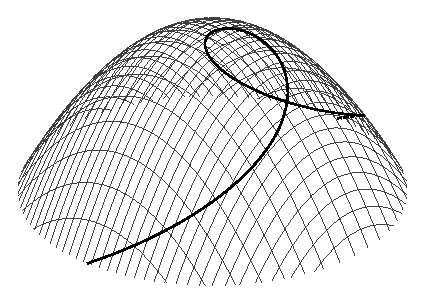
\includegraphics[width=8cm,height=8cm]{figures/parab}
  \end{center}

  \caption{\small Surface plotting with Gnuplot.}
  \label{fig-gnuplot}
\end{figure}

\lstset{frame=single, basicstyle=\small}
\mbox{
\lstinputlisting{figures/c_parabola}}


\section{Surfaces with \myindx{Google Sketchup}}
Google Sketchup is a 3D modelling tool provided free of charge. One cool 
feature of Sketchup is the API which makes it easy to write custom plugins 
for creating 3D graphics. In Sketchup we have fine control over colors, 
transparency, shadows, materials and because Sketchup is Polygon based it 
can also do hidden line removal. Put the following Ruby script in the Plugins 
folder and it will automatically run when you start Sketchup. The result is shown in figure \ref{fig-sketchup}.

\begin{figure}[!ht]
  \begin{center}
    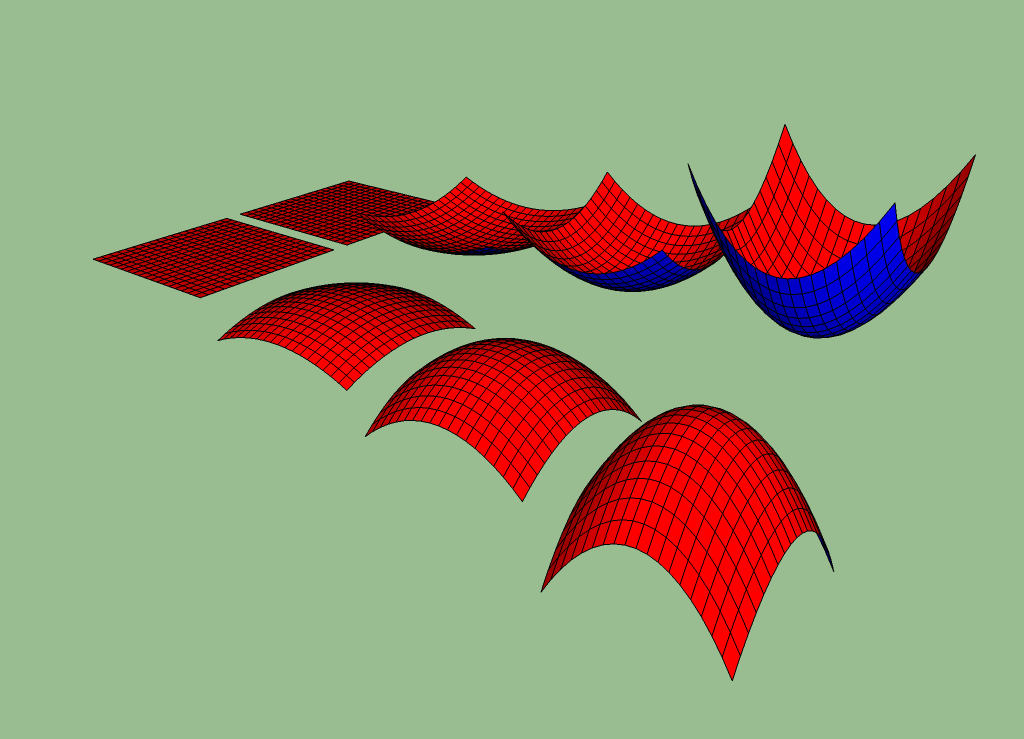
\includegraphics[width=12cm,height=12cm]{figures/rubyparabolas}
  \end{center}

  \caption{\small Plots generated by Google Sketchup plugin.}
  \label{fig-sketchup}
\end{figure}

\lstset{frame=single, basicstyle=\small}
\lstinputlisting{figures/parab.rb}


\section{\LaTeX, \myindx{\TikZ} and GNUPLOT}
If you feel the need for more graphical consistency in your mathematical
figures, you could use \TikZ which is a large framework for drawing graphics
within \LaTeX.

This ended up being my favorite because embedding the graphics allows
for a more coherent graphical representation with styles. Another 
advantage is that there is less hassle with including external 
plots and keeping these files up to date.

If The following lines of code are added to your document,



\begin{lstlisting}
  \begin{tikzpicture}[scale=2]
    \draw[step=.25cm,mjcgrid] (-0.74,-0.24) grid (3.4,2.4);
    \pgfsetlinewidth{1pt}

    \coordinate (o)  at (0,0);
    \coordinate (ox) at (3,0);
    \coordinate (oy) at (0,2);
    \draw [->] (o) -- (ox); 
    \draw [->] (o) -- (oy); 

    \node [right]  at (ox) {$\mathbf{x}$};
    \node [above]  at (oy) {$\mathbf{y}$};

    \draw[scale=0.5,domain=-3.141:3.141,smooth,red] 
          plot[parametric,prefix=pgffigs/mjc,id=par_test] 
          function{2+t*cos(t),1+t*sin(t)};
  \end{tikzpicture}
\end{lstlisting}

this figure will be produced. The key ``magic'' is the \textbf{draw ... plot} commands. 
\TikZ generates a gnuplot file, makes \LaTeX\ call GNUPLOT, which in turn generates
a file with a table of the computed values. These values are then read and presented 
in the graphical framework \TikZ produces.

\begin{center}
  \begin{tikzpicture}[scale=2]
    \draw[step=.25cm,mjcgrid] (-0.74,-0.24) grid (3.4,2.4);
    \pgfsetlinewidth{1pt}

    \coordinate (o)  at (0,0);
    \coordinate (ox) at (3,0);
    \coordinate (oy) at (0,2);
    \draw [->] (o) -- (ox); 
    \draw [->] (o) -- (oy); 

    \node [right]  at (ox) {$\mathbf{x}$};
    \node [above]  at (oy) {$\mathbf{y}$};

    \draw[scale=0.5,domain=-3.141:3.141,smooth,red] plot[parametric,prefix=pgffigs/mjc,id=par_test] 
            function{2+t*cos(t),1+t*sin(t)};
  \end{tikzpicture}
\end{center}


\section{Numerical integration}
For definite integrals of functions of one variable, \myindx{Romberg integration} was used. The program 
listed below is compiled and executed by the following commands

\command{gcc romberg.c} 

\command{./a.out}


\lstset{frame=single, basicstyle=\tiny}
\lstinputlisting{numerical/romberg.c}


\section{\myindx{Symbolic algebra} with Maxima}
\label{sec:maxima}

The following code written in Maxima, produces the output in section \ref{sec:maxima_sph}

\begin{lstlisting}
   load(ctensor);

   ct_coordsys([r*cos(theta)*cos(phi),r*cos(theta)*sin(phi),
      r*sin(theta),[r,theta,phi]]);

   lg:trigsimp(lg);

   christof(lcs);

   ug:invert(lg);

   christof(mcs);
\end{lstlisting}

